% !TEX root = saveliev_physics_general_course_1.tex
%!TEX TS-program = pdflatex
%!TEX encoding = UTF-8 Unicode

% \chapter{PHYSICAL KINETICS}\label{chap:16}
\chapter{ĐỘNG HỌC VẬT LÝ}\label{chap:16}
% \section{Transport Phenomena}\label{sec:16_1}
\section{Hiện tượng vận chuyển}\label{sec:16_1}
% Statistical physics has to do with equilibrium states and reversible processes (\ie, processes in which a system passes through a sequence of equilibrium states). The science studying the processes that are set up when equilibrium is violated is called \textbf{physical kinetics}.
Vật lý thống kê nghiên cứu các trạng thái cân bằng của các vật với những quá trình thuận nghịch(tức là những quá trình trong đó hệ đi qua một chuỗi những trạng thái cân bằng). Bộ môn khoa học nghiên cứu những quá trình được hình thành khi trạng thái cân bằng bị phá vỡ gọi là \textbf{động học vật lý}.

% When equilibrium of a system is violated, the system tends to return to its equilibrium state. This process is attended by a growth in entropy and is consequently irreversible. Thus, the processes which physical kinetics studies are irreversible.
Khi cân bằng bị phá vỡ, hệ có xu hướng trở về trạng thái cân bằng. Quá trình này được kèm theo bởi sự gia tăng của entropy và do đó không thuận nghịch. Vì vậy, những quá trình mà động học vật lý nghiên cứu là những quá trình không thuận nghịch.

% The violation of equilibrium is accompanied by the appearance of flows of either molecules, or heat, or an electric charge, and so on. In this connection, the relevant processes are called \textbf{transport phenomena}. It follows from the above that transport phenomena are irreversible processes.
Sự phá vỡ cân bằng được kèm theo bởi sự phát sinh những dòng hoặc phận tử, hoặc nhiệt, hoặc điện tích, v.v.. Do đó, những quá trình tương ứng được gọi là \textbf{hiện tượng vận chuyển}. Từ những điều trên ta suy ra hiện tượng vận chuyển là những quá trình không thuận nghịch.

Ta xét ba hiện tượng vận chuyển---sự khuếch tán, sự dẫn nhiệt, nội ma sát hay sự nhớt, đồng thời giới hạn ở những trường hợp mà sai lệch so với vị trí cân bằng là không đáng kể. Thoạt tiên, ta viết những phương trình thực nghiệm của các quá trình này, chúng có thể áp dụng được cho bất kỳ môi trường nào (rắn, lỏng, khí). Trong những mục sau, ta sẽ biểu diễn các phương trình của chất khí này theo quan điểm nhiệt học phân tử.

% When considering transport phenomena, we shall have to calculate the amounts of various quantities (the number of particles, mass, energy, momentum) transported through an imaginary surface. The amount of a quantity passing in unit time through a surface is called the \textbf{flux} (\textbf{flow}) of this quantity. Examples are the flux (flow) of a liquid through a cross section of a pipe or tube, and the light flux through a window pane or through the glass bulb of an electric lamp. We can consider the flux through a surface of any shape; in particular, the surface can be closed.
Khi nghiên cứu các hiện tượng vận chuyển, ta sẽ phải tính thêm số lượng của nhiều đại lượng khác nhau (số các hạt, khối lượng, năng lượng, động lượng) được truyền qua một mặt tưởng tượng nào đó. Số lượng của một đại lượng truyền qua mặt trong một đơn vị thời gian được gọi là \textbf{thông lượng} (\textbf{lưu lượng}) của đại lượng đó. Những ví dụ có thể kể đến là thông lượng (lưu lượng) của một chất lỏng qua tiết diện ngang của ống, thông lượng ánh sáng qua tấm kính cửa sổ hoặc qua cái bầu thủy tinh của bóng đèn điện. Có thể xét thông lượng xuyên qua một mặt có hình dạng tùy ý; đặc biệt, mặt ta chọn có thể là mặt kín.

% The flux is a scalar algebraic quantity. The sign of a flux is determined by the choice of the positive direction, for example, the direction of the axis along which the flux propagates. The positive direction is usually chosen arbitrarily. For closed surfaces, it is customary practice to consider the flux flowing out of the surface as positive, and that flowing into it as negative. In this chapter, we shall deal with fluxes through flat surfaces perpendicular to the $z$-axis. If particles, energy, or momentum will be transported through the surface in the direction of the $z$-axis, we shall consider the corresponding flux to be positive, otherwise we shall consider it negative.
Thông lượng là một đại lượng đại số và vô hướng. Dấu của thông lượng được xác định bằng cách chọn chiều dương, chẳng hạn bởi chiều của trục dọc mà theo đó thông lượng lan truyền. Chiều dương thông thường được chọn một cách tùy ý. Đối với những mặt kín, người ta quy ước thông lượng truyền qua mặt ra ngoài là dương, còn thông lượng truyền vào trong là âm. Trong chương này, ta nghiên cứu thông lượng qua những mặt phẳng vuông góc với trục $z$. Nếu các hạt, năng lượng hoặc động lượng được truyền qua mặt theo chiều của trục $z$ thì ta xem thông lượng tương ứng là dương, trong trường hợp ngược lại là âm.

% Every transport phenomenon is due to changes in a certain quantity $f$ in space. This quantity for the transport of particles (diffusion) is the concentration of the particles---the latter are transported in the direction of diminishing of their concentration. A heat flux appears when the temperature at different points of the medium differs, the heat flowing in the direction of diminishing temperature, etc.
Tát cả những hiện tượng vận chuyển được gây ra bởi biến thiên của một đại lượng $f$ bất kỳ trong không gian. Trong trường hợp vận chuyển hạt (khuếch tán), nồng độ các hạt là một đại lượng như vậy---nghĩa là sự vận chuyển các hạt được thực hiện theo chiều giảm nồng độ của chúng. Thông lượng nhiệt xuất hiện khi có sự chênh lệch nhiệt độ giữa các điểm khác nhau trong cùng một môi trường, hơn nữa nhiệt truyền theo chiều giảm của nhiệt độ, v.v..

% We shall consider for simplicity that the quantity $f$ whose lack of homogeneity underlies the given transport process (the concentration, temperature, etc.) is a function of only the coordinate $z$. Hence, the change in this quantity in space will he characterized by the derivative $\diffin{f}{z}$. The latter is usually called the gradient of the quantity $f$. This name is not quite correct---strictly speaking, the derivative of the scalar function $f=f(z)$ with respect to $z$ gives the projection of the gradient of the function onto the $z$-axis [see \eqn{3_23}]. Following the tradition, however, we shall call quantities of the kind $\diffin{f}{z}$ in a transport equation a \textbf{gradient}.
Để đơn giản, ta xem  đại lượng $f$ là hàm của chỉ tọa độ $z$. Sự không đồng nhất của $f$ chính là nguyên nhân của quá trình vận chuyển (nồng độ, nhiệt độ, v.v..) . Khi đó, sự biến thiên của đại lượng này trong không gian được đặc trưng bởi đạo hàm $\diffin{f}{z}$, hay thường được gọi là gradient của đại lượng $f$. Điều này là không quá chính xác---nói một cách chặt chẽ, đạo hàm của hàm vô hương $f=f(z)$ theo $z$ cho kết quả là hình chiếu gradient của $f$ lên trục $z$. Tuy nhiên, theo truyền thống, ta vẫn sẽ gọi các đại lượng dạng $\diffin{f}{z}$ trong các phương trình vận chuyển là \textbf{gradient}.

% \textbf{Diffusion.} Diffusion is defined as the spontaneous levelling out of the concentrations in a mixture of several (in the simplest case of two) different substances due to thermal motion. This process is observed in solid, liquid, and gaseous media. We shall consider only gaseous media.
\textbf{Sự khuếch tán.} Sự khuếch tán được định nghĩa là sự san bằng một cách tự phát nồng độ trong hỗn hợp của một vài (trong trường hợp đơn giản là hai) chất khác nhau, nó được gây ra bởi chuyển động nhiệt của các phân tử. Quá trình này được thấy ở cả môi trường rắn, lỏng và khí. Tuy nhiên, ta giới hạn chỉ xét ở môi trường khí.

%Assume that a unit volume of a two-component gas mixture contains $n_1$ molecules of one species and $n_2$ molecules of another one. The total number of molecules in unit volume is $n=n_1+n_2$. The ratio
% \begin{equation*}
   % c_i = \frac{n_i}{n}
% \end{equation*}
Giả sử trong một đơn vị thể tích của một hỗn hợp hai khí chứa $n_1$ phân tử loại này và $n_2$ phân tử loại kia. Tổng số phân tử trong một đơn vị thể tích là $n=n_1+n_2$. Tỷ số
\begin{equation*}
    c_i = \frac{n_i}{n}
\end{equation*}

% \noindent
được gọi là \textbf{nồng độ tỷ đối} của phần tử thứ $i$.

\begin{figure}[!htb]
	\begin{center}
		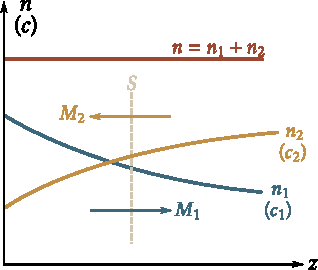
\includegraphics[scale=1]{figures/ch_16/fig_16_1.pdf}
		\caption[]{}
		\label{fig:16_1}
	\end{center}
\end{figure}

% Let us assume that concentration gradients $\diffin{c_1}{z}$ and $\diffin{c_2}{z}$ are set up in the direction of the $z$-axis, and $\diffin{c_1}{z}=-\diffin{c_2}{z}$ (\fig{16_1}). Hence,
Giả sử theo hướng của trục $z$ có các gradient nồng độ $\diffin{c_1}{z}$ và $\diffin{c_2}{z}$, hơn nữa $\diffin{c_1}{z}=-\diffin{c_2}{z}$ (\fig{16_1}). Khi đó,

\begin{equation*}
    \frac{\upd}{\deriv{z}}(c_1 + c_2) = \frac{1}{n}\frac{\upd}{\deriv{z}}(n_1 + n_2) = 0
\end{equation*}


\begin{figure}[!htb]
	\begin{center}
		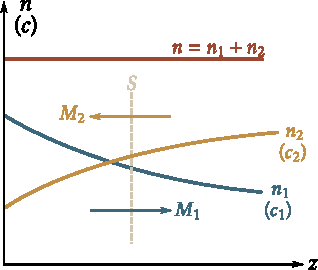
\includegraphics[scale=1]{figures/ch_16/fig_16_1.pdf}
		\caption[]{}
		\label{fig:16_1}
	\end{center}
\end{figure}

Cho nên $n$ và do đó cả $p$ đều không đổi ($p=nkT$). Vì vậy, các thông lượng khí động học không xuất hiện. Tuy nhiên, do chuyển động nhiệt của các phân tử, quá trình san bằng nồng độ sẽ diễn ra kèm theo chuyển động của mỗi đơn vị khối lượng theo chiều giảm dần nồng độ. Như đã nói ở trên, quá trình này được gọi là sự khuếch .

% It has been established experimentally that the flux of molecules of the $i$-th species through surface $S$ perpendicular to the $z$-axis is determined by the expression
Bằng thực nghiệm, thông lượng của phân tử thứ $i$ qua tiết diện $S$ vuông góc với trục $z$ được xác định bởi công thức
\begin{equation}\label{eq:16_1}
    N_i = -D \diff{n_i}{z} S
\end{equation}

\noindent
trong đó $D$ là một hằng số tỷ lệ và được gọi là \textbf{hệ số khuếch tán}.

% According to \eqn{16_1}, when $\diffin{n_i}{z}>0$, the flux $N_i$ is negative; this signifies that the molecules are transported in a direction opposite to that of the $z$-axis (\fig{16_2}a). When $\diffin{n_i}{z}<0$, the flux is positive, \ie, the molecules are transported in the direction of the $z$-axis (\fig{16_2}b). Thus, the minus sign in \eqn{16_2} is due to the fact that the molecules flow in the direction of diminishing of the concentration.
Theo \eqn{16_1}, trong trường hợp khi $\diffin{n_i}{z}>0$, thông lượng $N_i$ âm; điều đó có nghĩa các phân tử được vân chuyển ngược chiều dưởng của trục $z$ (\fig{16_2}a). Còn khi $\diffin{n_i}{z}<0$, thông lượng dương, các phân tử được vận chuyển theo chiều dương trục $z$ (\fig{16_2}b). Như vậy, dấu trừ trong \eqn{16_2} biểu thị rằng thông lượng các phân tử hướng theo chiều giảm của nồng độ.

% The dimension of the flux of molecules $N$ is T$^{-1}$, that of $n_i$ is L$^{3}$, of the area $S$ is L$^{2}$, and $\deriv{z}$ has the dimension L. Hence, the diffusion coefficient has the dimension L$^2$T$^{-1}$. Multiplying both sides of \eqn{16_1} by the mass of a molecule of the $i$-the species $m_i$ we get an expression for the flux of the mass of the $i$-th component:
Thứ nguyên của thông lượng các phân tử $N$ là T$^{-1}$, thứ nguyên của $n_i$ là L$^{3}$, của diện tích $S$ là L$^{2}$, và $\deriv{z}$ có thứ nguyên là L. Do đó, hệ số khuếch tán có thứ nguyên là L$^2$T$^{-1}$. Nhân cả hai vế của \eqn{16_1} với khối lượng $m_i$ của phân tử thứ $i$ ta thu được biểu thức về thông lượng của khối lương của thành phần thứ $i$:
\begin{equation}\label{eq:16_2}
    M_i = -D \diff{\rho_i}{z} S.
\end{equation}

\noindent
% Here $\rho_i=n_im_i$ is the partial density of the $i$-th component; it is also called the \textbf{absolute concentration}.
Trong đó $\rho_i=n_im_i$ là mật độ riêng phần của thành phần thứ $i$; nó còn được gọi là \textbf{nồng độ tuyệt đối}.

Phương trình ~\eqref{eq:16_1} và ~\eqref{eq:16_2} là những phương trình thực nghiệm của sự khuếch tán. Chúng còn được gọi là \textbf{Định luật Flick}.

\begin{figure}[!htb]
	\begin{center}
		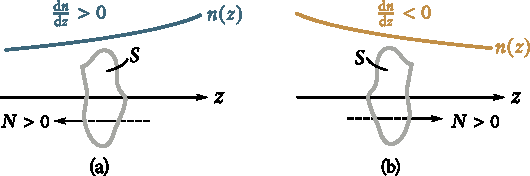
\includegraphics[scale=1]{figures/ch_16/fig_16_2.pdf}
		\caption[]{}
		\label{fig:16_2}
	\end{center}
\end{figure}

% \textbf{Thermal Conductivity.} Experiments show that if we set up a temperature gradient along the $z$-axis in a medium (solid, liquid, or gaseous one), then a heat flux is produced whose magnitude is determined by the formula
\textbf{Sự dẫn nhiệt.} Thực nghiệm cho thấy nếu ta tạo ra một gradient nhiệt độ dọc theo trục $z$ ở một môi trường (rắn, lỏng hoặc khí) thì xuất hiện một thông lượng nhiệt mà độ lớn của nó được xác định bởi công thức
\begin{equation}\label{eq:16_3}
    q = -\varkappa \diff{T}{z} S
\end{equation}

\noindent
% where $q$ is the heat flux through surface $S$ perpendicular to the $z$-axis, $\diffin{T}{z}$ is the temperature gradient (more exactly, the projection of the temperature gradient on the $z$-axis) and $\varkappa$ is a proportionality constant depending on the properties of the medium and called the \textbf{thermal conductivity coefficient}.
Ở đây $q$ là thông lượng nhiệt qua tiết diện $S$ vuông góc với trục $z$, $\diffin{T}{z}$ là gradient nhiệt độ (chính xác hơn, là hình chiếu của gradient nhiệt độ lên trục $z$) và $\varkappa$ là một hằng số tỷ lệ phụ thuộc vào tính chất của môi trường và được gọi là \textbf{hệ số dẫn nhiệt}.

% Đơn vị của $q$ là \si{\joule\per\second}, \ie, \si{\watt} (watt). Hence, $\varkappa$ is measured in watts per metre-kelvin $\bracket{\si{\watt\per\metre\per\kelvin}}$. The minus sign in \eqn{16_3} signifies that the heat flows in the direction of diminishing of the temperature. Therefore, the signs of $q$ and $\diffin{T}{z}$ are opposite. Equation~\eqref{eq:16_3} is an empirical equation of thermal conductivity. It is also called the \textbf{Fourier law}.
Đơn vị của $q$ là \si{\joule\per\second}, tức là \si{\watt} (watt). Do đó, $\varkappa$ được đo bằng watts trên metre-kelvin $\bracket{\si{\watt\per\metre\per\kelvin}}$. Dấu trừ trong \eqn{16_3} cho thấy nhiệt truyền theo chiều giảm của nhiệt độ. Vì vậy, $q$ trái dấu với $\diffin{T}{z}$. Phương trình~\eqref{eq:16_3} là một phương trình thực nghiệm về sự dẫn nhiệt. Nó còn được gọi là \textbf{Định luật Fourier}.

\textbf{Nội ma sát.} Theo \eqn{0.1.4}, lực ma sát giữa hai lớp chất lỏng hoặc chất khí là
\begin{equation}\label{eq:0.1.4}
    F = \eta \absolute{\diff{u}{z}} S
\end{equation}

\noindent
Trong đó $\eta$ là hệ số nhớt, $\diffin{u}{z}$ là đại lượng chỉ vận tốc của chất lỏng hoặc chất khí theo hướng của trục $z$ vuông góc với hướng chuyển động của các lớp ( gradient của $u$) và $S$ là tiết diện của mặt mà theo đó lực $F$ tác dụng.

% Equation~\eqref{eq:16_4} is the empirical equation of viscosity.
Phương trình ~\eqref{eq:0.1.4} là phương trình thực nghiệm của độ nhớt.

% According to Newton's second law, the interaction of two layers with the force $F$ can be considered as a process in the course of which a momentum equal to $F$ in magnitude is transmitted from one layer to another in unit time. Therefore, \eqn{0.1.4} can be written in the form
Theo định luật II Newton, tương tác giữa hai lớp mà lực $F$ tác dụng có thể coi như là quá trình mà lớp này truyền cho lớp kia một xung lượng có độ lớn $F$ trong một đơn vị thời gian. Vì vậy, có thể biểu diễn \eqn{0.1.4} dưới dạng
\begin{equation}\label{eq:16_5}
    K = -\eta \diff{u}{z} S
\end{equation}

\noindent
% where $K$ is the momentum transmitted in one second from layer to layer through surface $S$, \ie, the momentum flux through $S$.
Trong đó $K$ là xung lượng được truyền trong một giây từ lớp nọ sang lớp kia qua tiết diện $S$, tức là thông lượng xung lượng qua $S$.

% The momentum flux $K$ is measured in \si{\kilo\gram\metre\per\second\squared}. Hence, the unit of the viscosity $\eta$ is the kilogramme per metre-second $\bracket{[\si{\kilo\gram\per\metre\per\second}}$. [This unit can also be written in the form pascal-second (\si{\pascal\second}).]
Thông lượng xung lượng $K$ được đo theo đơn vị \si{\kilo\gram\metre\per\second\squared}. Vì vậy, đơn vị của hệ số nhớt $\eta$ là kilogramme trên metre-giây $\bracket{[\si{\kilo\gram\per\metre\per\second}}$. [Cũng có thể biểu diễn đơn vị đo này dưới dạng Pascal-giây (\si{\pascal\second}).]

% The minus sign in \eqn{16_5} is due to the circumstance that the momentum ``flows'' in the direction of the decrease in the velocity $u$. Therefore, the signs of the flux $K$ and of the derivative $\diffin{u}{z}$ are opposite.
Dấu trừ trong \eqn{16_5} thể hiện cho xung lượng "truyền" theo hướng giảm của vận tốc $u$. Vì vậy, dấu của thông lượng $K$ và của đạo hàm $\diffin{u}{z}$ là trái nhau.

% It must be remembered that \eqn{16_4} determines the identical modulus of two oppositely directed forces with which the layers act on each other. Therefore, the minus sign must not be written in front of the right-hand side of \eqn{16_4}. In addition, we must take the magnitude of the expression $\diffin{u}{z}$ (the magnitude of the force with any sign of the derivative $\diffin{u}{z}$ must be positive).
Nhớ lại rằng \eqn{0.1.4} xác định module của hai lực ngược chiều mà các lớp tác dụng lên nhau. Vì vậy, không đước viết dấu trừ trước về phải của \eqn{0.1.4}. Ngoài ra, cần lấy độ lớn của biểu thức $\diffin{u}{z}$ (độ lớn của lực với bất kỳ dấu nào của đạo hàm $\diffin{u}{z}$ đều phải là dương).

\section{Quãng Đường Tự Do Trung Bình}\label{sec:16_2}

% The molecules of a gas in thermal motion continuously collide with one another. The term ``collision'' as applied to molecules must not be understood literally and the process conceived as the collision of rigid balls. By a collision of molecules is meant the process of interaction between them as a result of which the molecules change the direction of their motion. 
Các phân tử khí chuyển động nhiệt liên tục va chạm với nhau. ``Va chạm'' trong chuyển động phân tử không nên được hiểu một cách máy móc mà ta nên hình dung nó như quá trình va chạm của các quả cầu rắn. Va chạm là quá trình tương tác giữa các phân tử mà kết quả của quá trình này chính là sự đổi hướng chuyển động của phân tử.

\begin{figure}[!htb]
	\begin{center}
		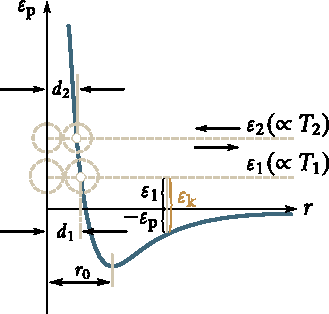
\includegraphics[scale=1]{figures/ch_16/fig_16_3.pdf}
		\caption[]{}
		\label{fig:16_3}
	\end{center}
\end{figure}

% Figure~\ref{fig:16_3} shows a curve depicting the mutual potential energy of two molecules as a function of the distance $r$ between their centres. Let us use this curve to consider the process of the approach (collision) of molecules. Let us mentally place the centre of one of the molecules at the origin of coordinates, and imagine the centre of the second molecule moving along the $r$-axis. Assume that the second molecule is flying toward the first one from infinity having the initial store of kinetic energy $\ab{\varepsilon}{k}=\varepsilon_1$. Approaching the first molecule, the second one under the action of the force of attraction moves with a constantly growing velocity. The kinetic energy of a molecule $\ab{\varepsilon}{k}$ also grows as a result. The total energy of the system equal to $\varepsilon=\ab{\varepsilon}{k}+\ab{\varepsilon}{p}$, however, remains unchanged (the system of the two molecules is closed) and equal to $\varepsilon_1$ because the potential energy $\ab{\varepsilon}{p}$ diminishes simultaneously. When the molecule passes the point with the coordinate $r_0$, the forces of attraction are replaced by forces of repulsion, owing to which the molecule begins to rapidly lose its velocity (in the region of repulsion the curve of $\ab{\varepsilon}{p}$ is very steep). At the moment when the potential energy $\ab{\varepsilon}{p}$ becomes equal to the total energy of the system $\varepsilon_1$, the velocity of the molecule vanishes. At this moment, the molecules approach each other to the closest distance. After the molecule stops, all the phenomena proceed in the reverse sequence: first the molecule travels with a constantly growing velocity under the action of the force of repulsion, upon covering the distance $r_0$, the molecule gets under the action of the force of attraction that retards its motion and, finally, travels away to infinity having its initial store of kinetic energy $\varepsilon_1$.
Hình ~\ref{fig:16_3} là đồ thị thế năng tương tác của hai phân tử, với biến số là khoảng cách giữa hai khối tâm phân tử. Ta sẽ sử dụng đồ thị này để nghiên cứu về sự tiếp cận (va chạm) của các phân tử. Ta đặt gốc toạ độ tại khối tâm của một phân tử, còn khối tâm của hạt còn lại thì dịch chuyển dọc theo trục r. Giả sử phân tử thứ hai đang chuyển động từ xa vô cùng về phía phân tử thứ nhất, với động năng ban đầu là $\ab{\varepsilon}{k}=\varepsilon_1$. Khi di chuyển tới phân tử thứ nhất, tốc độ của phân tử thứ hai tăng dần, đồng nghĩa với động năng của phân tử hai, $\ab{\varepsilon}{k}$, cũng tăng lên. Năng lượng toàn phần của hệ là $\varepsilon=\ab{\varepsilon}{k}+\ab{\varepsilon}{p}$ không đổi (hệ hai phân tử là hệ kín) và bằng $\varepsilon_1$, vì thế nên thế năng tương tác $\ab{\varepsilon}{p}$ sẽ giảm dần. Khi toạ độ của phân tử hai là $r_0$, lực hút sẽ được thay thế bằng lực đẩy, do đó vận tốc của phân tử sẽ giảm rất nhanh (Trong vùng xuất hiện lực đẩy, thì đường cong của $\ab{\varepsilon}{p}$ rất dốc). Tại thời điểm mà thế năng $\ab{\varepsilon}{p}$ bằng với tổng năng lượng hệ $\varepsilon_1$, vận tốc của phân tử sẽ bị triệt tiêu. Cùng lúc đó, khoảng cách giữa hai phân tử nhỏ nhất. Khi các phân tử dừng lại, thì hiện tượng diễn ra theo chiều ngược lại: đầu tiên, dưới tác động của lực đẩy, vận tốc của phân tử tăng dần; khi đi qua toạ độ $r_0$, phân tử chịu tác động của lực hút làm hãm chuyển động của hạt (vận tốc giảm dần); và cuối cùng đi ra xa vô cùng với động năng bằng đúng động năng ban đầu $\varepsilon_1$.


% The minimum distance between the centres of two molecules when they collide is called the \textbf{effective} or \textbf{collision diameter} of a molecule $d$ (\fig{16_4}). The quantity
Khoảng cách nhỏ nhất giữa tâm của hai phân tử được gọi là \textbf{đường kính hiệu dụng}\footnote{Còn có một cách gọi khác cho đại lượng $d$ là \textbf{đường kính va chạm} của phân tử.} $d$ của phân tử (\fig{16_4}). Đại lượng 
\begin{equation}\label{eq:16_6}
    \sigma = \pi d^2
\end{equation}

\noindent
% is known as the effective section of a molecule.
được gọi là \textbf{tiết diện hiệu dụng} của phân tử.

\begin{figure}[!htb]
	\begin{center}
		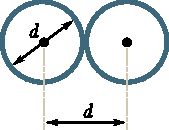
\includegraphics[scale=1]{figures/ch_16/fig_16_4.pdf}
		\caption[]{}
		\label{fig:16_4}
	\end{center}
\end{figure}

% A glance at \fig{16_3} shows that when a molecule begins its motion from infinity with a greater store of energy, the minimum distance between the centres of the molecules when they approach is less (compare $d_1$ and $d_2$ in the figure). Thus, the collision diameter of molecules depends on their energy and, consequently, on the temperature. The collision diameter of molecules diminishes with increasing temperature.
Từ \fig{16_3} có thể thấy, khi trữ lượng năng lượng (động năng ở xa vô cùng) của phân tử càng lớn, thì khoảng cách nhỏ nhất giữa hai tâm phân tử càng nhỏ (so sánh $d_1$ và $d_2$ trong hình). Vậy, đường kính hiệu dụng của phân tử phụ thuộc vào năng lượng của hệ và do đó cũng phụ thuộc vào nhiệt độ. Khi nhiệt độ tăng cao thì đường kính hiệu dụng giảm.

% During one second, a molecule travels an average path equal to the mean velocity $\average{v}$. If it experiences an average of $\nu$ collisions a second, then the mean free path will be
Trong một giây, một phân tử di chuyển được một quãng đường trung bình bằng với vận tốc trung bình $\average{v}$. Nếu như trong một giây, nó va chạm trung bình $\nu$ lần thì quãng đường tự do trung bình\footnote{quãng đường của phân tử đi được trước khi bị va chạm với một phân tử khác.} là
\begin{equation}\label{eq:16_7}
    l = \frac{\average{v}}{\nu}.
\end{equation}

% To calculate the average number of collisions $\nu$, let us first assume that all the molecules except for a given one are frozen still in their places. Let us watch the motion of the molecule we have earmarked. After striking one of the stationary molecules, it will fly in a straight line until it collides with another stationary molecule (\fig{16_5}). This collision will occur if the centre of the stationary molecule is at a distance from the line of flight of the molecule less than the collision diameter of a molecule $d$. As a result of the collision, the molecule will change the direction of its motion, and will then again fly along a straight line for a time. This will continue until it encounters another molecule whose centre will be within the cylinder of radius $d$ shown in \fig{16_5}.
Để tính toán số va chạm trung bình $\nu$, trước tiên hãy giả định rằng tất cả các phân tử khác, ngoại trừ phân tử đang xét, đều cố định. Giờ ta xét chuyển động của phân tử đã giả định ở trên. Sau khi va chạm với một phân tử, nó sẽ chuyển động trên đường thẳng tới va chạm với một phân tử cố định kế tiếp (\fig{16_5}). Va chạm diễn ra khi khoảng cách giữa phân tử cố định và phân tử chuyển động nhỏ hơn đường kính hiệu dụng $d$. Kết quả sau va chạm là phân tử đổi hướng chuyển động, và tiếp tục chuyển động thẳng trong một quãng thời gian. Điều này sẽ lặp lại khi mà phân tử chuyển động gặp một phân tử cố định có tâm nằm trong phạm vi hình trụ với bán kính $d$\footnote{Hình trụ này là kết quả khi tiết diện va chạm quét một vùng trong không gian, bất cứ hạt nào có tâm thuộc phạm vi hình trụ đều có khả năng va chạm.} như hình \fig{16_5}.

% The molecule travels a path of $\average{v}$ in one second. The number of collisions with stationary molecules occurring during this time equals the number of molecules whose centres are within the bent cylinder of length $\average{v}$ and radius $d$. It will be shown below that the mean free path is much larger than the collision diameter of the molecules $d$. Therefore, the volume of the cylinder can be considered equal to $\pi d^2\average{v}$. Multiplying this volume by the number of molecules in a unit volume $n$, we get the average number of collisions of a moving molecule with stationary ones per second:
Một phân tử di chuyển trong một giây được quãng đường bằng $\average{v}$. Số va chạm với các phân tử cố định trong khoảng thời gian này bằng số phân tử có tâm thuộc vào hình trụ gấp khúc với tổng độ dài $\average{v}$ và bán kính $d$. Dưới đây chứng tỏ rằng quãng đường tự do trung bình lớn hơn rất nhiều so với đường kính hiệu dụng $d$. Do đấy, thể tích của khối trụ bằng $\pi d^2\average{v}$. Nhân thể tích mới tìm được với mật độ hạt trên một đơn vị thể tích $n$, chúng ta sẽ có số va chạm trung bình của một phân tử chuyển động với các phân tử cố định khác, trong khoảng thời gian một giây.
\begin{equation}\label{eq:16_8}
    \nu' = \pi d^2 \average{v} n.
\end{equation}

\begin{figure}[!htb]
	\begin{center}
		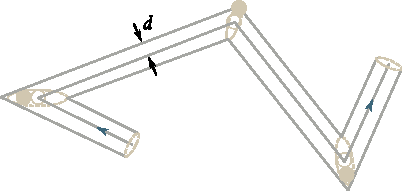
\includegraphics[scale=1]{figures/ch_16/fig_16_5.pdf}
		\caption[]{}
		\label{fig:16_5}
	\end{center}
\end{figure}

%Actually, all the molecules are in motion, owing to which the number of collisions is determined by the mean velocity of motion of the molecules with respect to one another, and not by the mean velocity $\average{v}$ of molecules relative to the walls of the vessel confining them. The relative velocity of two arbitrarily taken molecules is 
Thực tế, tất cả các phân tử đều chuyển động, nên số va chạm được tính bằng vận tốc trung bình của các phân tử đối với nhau, chứ không phải vận tốc trung bình đối với thành bình $\average{v}$. Vận tốc tương đối giữa hai phân tử bất kì là
\begin{equation*}
    \ab{\vec{v}}{rel} = \vec{v}_2 - \vec{v}_1.
\end{equation*}

\noindent
%Squaring this equation, we get
Bình phương hai vế, ta có được

\begin{equation*}
    \ab{v}{rel}^2 = \parenthesis{\vec{v}_2 - \vec{v}_1}^2 = v_2^2 + v_1^2 - 2\vec{v}_1\vec{v}_2
\end{equation*}

\noindent
% (we have taken advantage of the fact that $\vec{v}^2=v^2$). The mean value of the sum of several quantities equals the sum of the mean values of the quantities being added. Hence,
(Chúng ta đã sử dụng sự thật là $\vec{v}^2=v^2$). Giá trị trung bình của một tổng các phần tử, bằng tổng của trung bình các phần tử ấy. Vì thế 
\begin{equation*}
    \average{\ab{v}{rel}^2} = \average{v_2^2} + \average{v_1^2} - 2\average{\vec{v}_1\vec{v}_2}.
\end{equation*}

\noindent
% Events consisting in that a first molecule has the velocity $\vec{v}_1$ and a second one the velocity $\vec{v}_2$ are statistically independent. Therefore, $\average{\vec{v}_1\vec{v}_2}=\average{\vec{v}_1}\average{\vec{v}_2}$. Each of the multipliers equals zero for a gas in equilibrium. Thus, 
Về mặt thống kê, biến cố mà phân tử thứ nhất có vận tốc $\vec{v}_1$ hoàn toàn độc lập với biến cố phân tử thứ hai có vận tốc $\vec{v}_2$. Vì thế, $\average{\vec{v}_1\vec{v}_2}=\average{\vec{v}_1}\average{\vec{v}_2}$. Đối với chất khí ở trạng thái cân bằng, thì mỗi thừa số bằng không. Vì vậy,
\begin{equation*}
    \average{\ab{v}{rel}^2} = \average{v_2^2} + \average{v_1^2} = 2\average{v^2}
\end{equation*}

\noindent
% (the mean value of the square of the velocity of all the molecules is the same and equals $\average{v^2}$). The result obtained signifies that $\ab{v}{rel,m. sq}=\sqrt{2}\ab{v}{m. sq}$. The mean square velocities are proportional to the arithmetical mean ones. Consequently,
(giá trị trung bình của bình phương vận tốc các phân tử tuỳ ý là bằng nhau và bằng $\average{v^2}$). Kết quả thu được là $\ab{v}{rel,m. sq}=\sqrt{2}\ab{v}{m. sq}$ \footnote{$\ab{v}{m. sq}$ có ý nghĩa là căn bậc 2 của trung bình bình phương vận tốc, $\sqrt{\average{v^2}}$ (m. sq = mean square) }. Trung bình của bình phương vận tốc sẽ tỉ lệ với bình phương trung bình vận tốc. Do đó,
\begin{equation*}
    \average{\ab{v}{rel}} = \sqrt{2}\average{v}.
\end{equation*}

%Substituting $\average{\ab{v}{rel}}$ for $\average{v}$ in \eqn{16_8}, we get the following expression for the mean number of collisions:
Thay thế $\average{v}$ bằng $\average{\ab{v}{rel}}$ trong \eqn{16_8}, chúng ta có biểu thức số va chạm trung bình: 
\begin{equation}\label{eq:16_9}
    \nu = \sqrt{2}\pi d^2 \average{v} n.
\end{equation}

\noindent
%Using this value of $\nu$ in \eqn{16_7}, we get the following equation for the mean free path:
Sử dụng giá trị $\nu$ trong \eqn{16_7}, chúng ta có công thức cho quãng đường tự do trung bình:
\begin{equation}\label{eq:16_10}
    l = \frac{1}{\sqrt{2}\pi d^2 n}.
\end{equation}

\noindent
%Substituting $\sigma$ for $\pi d^2$ in the above equation in accordance with \eqn{16_6}, we get
Từ \eqn{16_6} ta thay giá trị $\sigma$ bằng $\pi d^2$ vào công thức trên, ta sẽ thu được
\begin{equation}\label{eq:16_11}
    l = \frac{1}{\sqrt{2}\sigma n}.
\end{equation}

%At constant temperature, $n$ is proportional to $p$. Hence, the mean free path is inversely proportional to the pressure:
Tại một nhiệt độ không đổi, $n$ tỉ lệ thuật với $p$. Điều đó có nghĩa là quãng đường tự do trung bình tỉ lệ nghịch với áp suất:
\begin{equation}\label{eq:16_12}
    l \propto \frac{1}{p}.
\end{equation}

\noindent
% We noted above that the collision diameter of molecules diminishes with increasing temperature. Accordingly, elevation of the temperature is attended by an increase in the free path.
Chúng ta đã đề cập rằng đường kính hiệu dụng của phân tử giảm khi tăng nhiệt độ. Do đó, khi tăng nhiệt, quãng đường tự do trung bình tăng.

% Let us assess the value of the mean free path and the average number of collisions a second. We established in \sect{10_2} that molecules have dimensions of the order of several angstroms. Let us adopt the collision diameter of a molecule equal to \SI{2}{\angstrom}, \ie, \SI{2e-10}{\metre}. A mole of a gas in standard conditions (\ie, at \SI{0}{\degreeCelsius} and $p=\SI{1}{\atm}$) occupies a volume of \SI{22.4e-3}{\metre\cubed}. The number of molecules in unit volume in these conditions is $\num{6e23}/\num{22.4e-3}\approx\SI{3e25}{\per\metre\cubed}$. Introducing these numbers into \eqn{16_10}, we have 
Ta hãy ước lượng độ lớn của quãng đường tự do trụng bình và số va chạm trong một giây. Chúng ta đã chứng minh trong \sect{10_2} rằng kích thước phân tử cỡ một vài angstroms. Ta chọn đường kính hiệu dụng bằng \SI{2}{\angstrom}, hay \SI{2e-10}{\metre}. Một mol khí ở điều kiện tiêu chuẩn ( tại \SI{0}{\degreeCelsius} and $p=\SI{1}{\atm}$) có thể tích \SI{22.4e-3}{\metre\cubed}. Số va chạm trong một đơn vị thể tích xét trong điều kiện trên là $\num{6e23}/\num{22.4e-3}\approx\SI{3e25}{\per\metre\cubed}$. Thay vào \eqn{16_10}, ta có
\begin{equation*}
    l = \frac{1}{\sqrt{2}\times 3.14\times \num{4e-20}\times\num{3e25}} \approx \SI{2e-7}{\metre} = \SI{2e-5}{\centi\metre}.
\end{equation*}

%At a pressure of \SI{e-3}{\mmHg} (which corresponds to about \SI{e-6}{\atm}), $l$ will be of the order of \SI{10}{\centi\metre}. If a vessel has dimensions of a few centimetres, then at such a pressure the molecules will travel from wall to wall virtually without colliding with one another. At a pressure of \SI{e-6}{\mmHg} $l$ reaches a value of scores of metres.
Tại áp suất bằng \SI{e-3}{\mmHg} ( tương ứng với khoảng \SI{e-6}{\atm}), $l$ sẽ có độ lớn vào cỡ \SI{10}{\centi\metre}. Nếu bình chứa có kích thước vài centimet, thì tại áp suất đó các phân tử sẽ di chuyển từ thành này sang thành khác mà không va chạm với nhau. Tại áp suất \SI{e-6}{\mmHg} $l$ có độ lớn cỡ vài chục mét. 

%When deriving \eqn{16_8}, we assumed that $l$ is much greater than $d$. Now we can see that this assumption is correct. Indeed, it follows from the above assessment that in standard conditions the ratio of $l$ to $d$ is about $\num{2e-5}/\num{2e-10} = \num{e5}$.
Khi dẫn ra \eqn{16_8}, ta đã giả thiết rằng $l$ rất lớn so với $d$. Giờ chúng ta đã kiểu chứng giả thiết ấy. Khi đánh giá các giá trị tại điều kiện tiêu chuẩn thì tỉ số của $l$ trên $d$ là $\num{2e-5}/\num{2e-10} = \num{e5}$.

%We can find the number of collisions a second by dividing the mean velocity of the molecules $\average{v}$ by $l$. In \sect{11_6}, we obtained a value of $\average{v}$ of about \SI{500}{\metre\per\second} for oxygen. Dividing this value by $l=\SI{2e-7}{\metre}$, we get a value of \SI{2.5e9}{\per\second} for the number of collisions a second. Thus, in standard conditions, the number of collisions a second is several thousand millions. The number of collisions diminishes with a decreasing pressure, changing in proportion to $p$ [see \eqn{16_12}]. 
Chúng ta có thể tìm số va chạm trong một giây bằng cách chia vận tốc trung bình $\average{v}$ với $l$. Trong \sect{11_6}, chúng ta đã tính được giá trị của $\average{v}$ đối với khí oxy là \SI{500}{\metre\per\second}. Chia giá trị này cho $l=\SI{2e-7}{\metre}$, thì ta có số va chạm trong một giây là \SI{2.5e9}{\per\second}. Như ta thấy, trong điều kiện tiêu chuẩn, số chạm chạm có thể lên tới vài trăm triệu. Số va chạm giảm khi khi giảm áp suất, nó biến thiên tỉ lệ nghịch với $p$ [xem \eqn{16_12}].

% \section{Diffusion in Gases}\label{sec:16_3}
\section{Sự khuếch tán trong các chất khí}\label{sec:16_3}

% We shall attempt to get an equation of diffusion proceeding from molecular-kinetic notions. To simplify our task, we shall consider that the molecules of both components differ only slightly in mass ($m_1\approx m_2\approx m$) and have virtually identical effective sections ($\sigma_1\approx\sigma_2\approx\sigma$). In this case, we can assign the same mean velocity of thermal motion $\average{v}$ to the molecules of both components and calculate the mean free path by the equation
Ta sẽ thử tìm phương trình về sự khuếch tán bằng cách xuất phát từ các khái niệm về động học phân tử. Để đơn giản, ta xem các phân tử của cả hai thành phần có khối lượng khác nhau rất nhỏ ($m_1\approx m_2\approx m$) và hầu như có cùng một tiết diện hiệu dụng ($\sigma_1\approx\sigma_2\approx\sigma$). Trong trường hợp này, ta có thể coi các phân tử của cả hai thành phần có cùng vận tốc chuyển động nhiệt trung bình $\average{v}$ còn tính quãng đường tự do trung bình theo công thức
\begin{equation*}
    l = \frac{1}{\sqrt{2}\sigma n}
\end{equation*}

\noindent
Trong đó $n=n_1+n_2$.

% It is easy to understand that the process of diffusion in gases will proceed more intensively when the molecules have a higher velocity $\average{v}$ and collide less frequently with one another (\ie, the free path $l$ is greater). Consequently, we can expect that the diffusion coefficient $D$ must be proportional to the product $\average{v}l$. This agrees with the fact that, as we noted in \sect{16_1}, the dimension of $D$ is L$^2$T$^{-1}$.
Dễ hiểu rằng quá trinh khuếch tán trong các chất khí diễn ra càng mạnh khi phân tử chuyển động càng nhanh (nghĩa là khi $\average{v}$ càng lớn) cũng như khi chúng va chạm nhau càng thưa (tức là quãng đường tự do $l$ càng lớn). Do đó, có thể thừa nhận rằng hệ số khuếch tán $D$ tỷ lệ với thể tích $\average{v}l$. Điều này đồng nghĩa rằng, như đã nói ở \sect{16_1}, thứ nguyên của $D$ là L$^2$T$^{-1}$.

\begin{figure}[!htb]
	\begin{center}
		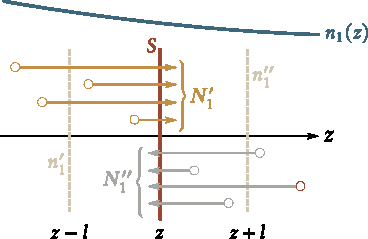
\includegraphics[scale=1]{figures/ch_16/fig_16_6.pdf}
		\caption[]{}
		\label{fig:16_6}
	\end{center}
	\vspace{-0.8cm}
\end{figure}

% Let us begin our calculations. Assume that the change in the concentration of the first component along the $z$-axis is described by the function $n_1=n_1(z)$. Let us denote the number of molecules of the first component flying through area $S$ in the direction of the $z$-axis a second by $N_1'$, and the number of molecules flying in the direction opposite to the $z$-axis by $N_1''$ (\fig{16_6})\footnote{We have drawn \fig{16_6} so that the molecules $N_1'$ fly through the upper half and the molecules $N_1''$ through the lower half of area $S$. Actually, both groups of molecules are distributed over the entire surface $S$.}. The difference between these numbers is the flux of the molecules of the first component $N_1$ through surface $S$:
Ta bắt đầu tính toán. Giả sử biến thiên nồng độ của thành phần thứ nhất dọc theo trục $z$ được mô tả bởi hàm $n_1=n_1(z)$. Ký hiệu số phân tử của thành phần thứ nhất qua tiết diện $S$ theo chiều của trục $z$ trong một giây là $N_1'$, và số phân tử theo chiều ngược lại là $N_1''$ (\fig{16_6})\footnote{Ta đã vẽ \fig{16_6} sao cho các phân tử $N_1'$ bay lên trên còn $N_1''$ bay xuống nửa dưới của tiết diện $S$. Thực tế, cả hai tập hợp phân tử phân bố theo toàn mặt $S$} Hiệu của hai số trên là thông lượng các phân tử của thành phần thứ nhất $N_1$ qua tiết diện $S$:
\begin{equation}\label{eq:16_13}
    N_1 = N_1' - N_1''.
\end{equation}

% We shall proceed from the simplified notion according to which the molecules move along three mutually perpendicular directions coinciding with the axes $x, y, z$ (the axes $x$ and $y$ are parallel to area $S$). In this case according to \eqn{11_24}, the number of molecules flying one of the directions through unit area a second is $n\average{v}/6$. Hence, the numbers $N_1'$ and $N_1''$ can be represented in the form
Ta sẽ bắt đầu từ khái niệm được đơn giản hóa, theo đó các phân tử chuyển động dọc theo ba trục vuông góc $x, y, z$ (trục $x$ và $y$ song song với tiết diện $S$). Trong trường hợp này, theo \eqn{11_24}, số phân tử xuyên qua một đơn vị diện tích theo một hương trong một giây là $n\average{v}/6$. Do đó các số $N_1'$ và $N_1''$ có thể được biểu diễn dưới dạng
\begin{equation}\label{eq:16_14}
    N_1' = \frac{1}{6}n_1'\average{v} S,\quad N_1'' = \frac{1}{6}n_1''\average{v} S.
\end{equation}

\noindent
% where $n_1'$ is the ``effective'' concentration of the molecules of the first component to the left of $S$, $n_1''$ is the same to the right of $S$.
Trong đó  $n_1'$ là nồng độ ``hiệu dụng'' của phân tử thành phấn thứ nhất phía bên trái $S$, còn $n_1''$ là của thành phân bên phải $S$.

% Molecules will fly through surface $S$ that experienced their last collision at different distances from it. On an average, however, the last collision will occur at a distance from $S$ equal to the mean free path $l$. It is therefore reasonable to take the value $n_1(z-l)$ as $n_1'$, and $n_1(z+l)$ as $n_1''$ (see \fig{16_6}). Hence, with a view to Eqs.~\eqref{eq:16_13} and~\eqref{eq:16_14}, we can write that
Các phân tử sẽ xuyên qua tiết diện $S$ sau khi va chạm tại những vị trí cách $S$ những khoảng khác nhau. Tuy nhiên, trung bình, va chạm cuối cùng nằm cách $S$ một khoảng bằng quãng đường tự do trung bình $l$. Vì vậy có thể lấy $n_1(z-l)$ là $n_1'$, và $n_1(z+l)$ là $n_1''$ (see \fig{16_6}). Do đó, quan sát Eqs.~\eqref{eq:16_13} và~\eqref{eq:16_14}, ta có thể viết thành
\begin{equation}\label{eq:16_15}
    N_1 = \frac{1}{6}\average{v} S [n_1(z-l) - n_1(z+l)].
\end{equation}

% Since $l$ is very small, the difference between the values of the function $n_1(z)$ given in \eqn{16_15} in brackets can be written in the form\footnote{Equation~\eqref{eq:16_16} holds provided that the change in $n_1$ over the free path is much smaller than $n_1$ itself $(\diffin{n_1}{z}l\leqslant n_1)$. This condition gives a criterion for the smallness of the deviation from equilibrium (see the fourth paragraph of \sect{16_1}). This remark relates to similar formulas of the following two sections. For example, \eqn{16_23} holds provided that $\diffin{T}{z}l\leqslant T$.}
Do $l$ rất nhỏ, hiệu giá trị của hàm $n_1(z)$ có thể viết là phần trong ngoặc vuông của \eqn{16_15} dưới dạng \footnote{Equation~\eqref{eq:16_16} vấn đúng trong trường hợp độ biến thiên của $n_1$ khi quãng đường tự do thay đổi là rất nhỏ so với chinh $n_1$  $(\diffin{n_1}{z}l\leqslant n_1)$. Từ đây ta được điều kiện về độ sai lệch khỏi trạng thái cân bằng (xem đoạn bốn của \sect{16_1}). Nhận xét này cũng đúng cho các công thức tương tự của hai mục sau đây. Ví dụ, \eqn{16_23} vẫn đúng trong điều kiện $\diffin{T}{z}l\leqslant T$.}
\begin{equation}\label{eq:16_16}
    n_1(z-l) - n_1(z+l) = - \diff{n_1}{z}2l.
\end{equation}

\noindent
% Introducing this expression into \eqn{16_15}, we find that
Thế biểu thức này vào \eqn{16_15}, ta được
\begin{equation}\label{eq:16_17}
    N_1 = - \parenthesis{\frac{1}{3} \average{v} l}\diff{n_1}{z} S.
\end{equation}

% A comparison of Eqs.~\eqref{eq:16_1} and~\eqref{eq:16_17} shows that on the basis of molecular-kinetic notions we can not only arrive at a proper dependence of $N_1$ on $\diffin{n_1}{z}$, but also obtain an expression for the diffusion coefficient $D$. This expression has the form
So sánh Eqs.~\eqref{eq:16_1} và ~\eqref{eq:16_17}, ta thấy rằng bằng các khái nhiệm động học phân tử, ta không những đưa tới sự phụ thuộc của $N_1$ vào $\diffin{n_1}{z}$ một cách chính xác, mà còn thu được biểu thức của hệ số khuếch tán $D$. Biểu thức đó có dạng
\begin{equation}\label{eq:16_18}
    D = \frac{1}{3} \average{v} l. 
\end{equation}

\noindent
% More strict calculations lead to the same formula, but with a somewhat different numerical factor.
Những tính toán kỹ càng hơn sẽ cho công thức tương tự, nhưng với một vài sai số nhỏ.

% It must be noted that as we assumed, the diffusion coefficient is proportional to the product $\average{v}l$.
Chý ý rằng ta đã giả thiết hệ số khuếch tán phụ thuộc vào tích $\average{v}l$.

% The derivation that led us to \eqn{16_17} can be applied with equal rights to both components of a mixture. Hence, the diffusion coefficient has the same value for both components.
Các bước thiết lập phương trình \eqn{16_17} cũng có thể được áp dụng tương tự cho cả hai thành phần của hỗn hợp. Do đó, hệ số khuếch tán của cả hai thành phần có giá trị như nhau.

% Let us investigate the expression we have obtained for the diffusion coefficient $D$. Inserting in \eqn{16_18} the expressions for $\average{v}$ and $l$, we find that
Xét biểu thức vừa thu được về hệ số khuếch tán $D$. Thế biểu thức của $\average{v}$ và $l$ vào \eqn{16_18}, ta được
\begin{equation}\label{eq:16_19}
    D \propto \frac{1}{n\sigma} \parenthesis{\frac{T}{m}}^{1/2}.
\end{equation} 

\noindent
% It follows from \eqn{16_9} that the diffusion coefficient is inversely proportional to the number of molecules in a unit volume, and, consequently, to the pressure $p$:
Từ \eqn{16_9} suy ra hệ số khuếch tán tỉ lệ nghịch với số phân tử trong một đơn vị thể tích và do đó tỉ lệ nghịch với áp suất $p$:
\begin{equation*}
    D \propto \frac{1}{p}.
\end{equation*}

\noindent
% With elevation of the temperature, $D$ grows approximately in proportion to $\sqrt{T}$ (we remind our reader that $\sigma$ slightly depends on $T$).
Khi nhiệt độ tăng, $D$ tăng gần như xấp xỉ tỉ lệ với $\sqrt{T}$ (nhớ rằng $\sigma$ phụ thuốc rất ít vào $T$).

% We have assumed that the molecules of both components are identical in mass and effective section. Therefore, \eqn{16_18} is in essence an expression for the coefficient of self-diffusion, \ie, the diffusion of the molecules of a gas in a medium containing molecules of the same gas. The phenomenon of self-diffusion could be observed if we marked in some way or other part of the molecules of a homogeneous gas. If the concentrations of marked molecules and of the molecules bearing no marks were not constant, counterflows of the two kinds of molecules would appear in the gas, and the magnitude of the flows would be determined by \eqn{16_17}. Self-diffusion can be studied in practice by employing the tracer technique. It consists in using a mixture of isotopes, \ie, varieties of atoms of the same element differing from each other, for example, in that one variety of the atoms is radioactive and the other is stable.
Ta đã giả thiết rằng các phân tử của cả hai thành phần có khối lượng và tiết diện hiệu dụng như nhau. Vì vậy, \eqn{16_18} thực chất là biểu thức của hệ số tự khuếch tán, \ie, tức là sự khuếch tán của phân tử một chất khí trong môi trường chứa các phân tử của cùng chất khí đó. Ta có thể quan sát hiện tượng tự khuếch tán bằng cách đánh dấu một phần trong số các phần tử của một chất khí đồng tính. Nếu như nồng độ của các phân tử đã được đánh dấu và của phần còn lại đề thay đổi, trong chất khí sẽ xuất hiện những thông lượng ngược nhau của hai phân tử khác loại, đồng thợi độ lớn của các thông lượng được xác định bởi công thức \eqn{16_17}. Thực tế có thể quan sát được hiện tượng tự khuếch tán bằng kĩ thuật đánh dấu. Phương pháp đó sử dụng hỗn hợp các đồng vị, \ie, tức là các biến thể nguyên tử của cùng một nguyên tố, chẳng hạn, một đồng vị có tính phóng xạ, còn đồng vị kia có tính bền vững.

Trong trường hợp có sự khác nhau trong khối lượng và tiết diện hiệu dụng của các phân tử cả hai thành phần, hệ số khuếch tán được xác định bởi công thức
\begin{equation*}
    D = \frac{n_1\average{v_2}l_2 + n_2\average{v_1}l_1}{3\parenthesis{n_1 + n_2}}
\end{equation*}

\noindent
% where $n_1, \average{v_1}, l_1$ are the concentration, mean velocity and mean free path of the molecules of the first component, and $n_2, \average{v_2}, l_2$ represent the same quantities for the molecules of the second component.
trong đó $n_1, \average{v_1}, l_1$ lần lượt là nồng độ, vận tốc trung bình và quãng đường tự do trung bình của các phân tử thành phần thức nhất, còn $n_2, \average{v_2}, l_2$ là các đại lượng tương tự của các phân tử thành phần thứ hai.

\section{Độ Dẫn Nhiệt của các Chất Khí}\label{sec:16_4}

%Let us calculate the heat flux in a gas on the basis of molecular-kinetic notions. If the temperature of the gas differs at different points, then the mean energy of the molecules at these points will also differ. Being displaced owing to thermal motion from one set of points to another, the molecules transport the energy they have stored. This energy transfer underlies the process of thermal conductivity in gases. Before beginning our calculations, let us attempt to reveal the factors that can affect the ability of a gas to conduct heat. It is easy to understand that apart from the factors determining the rate of diffusion, \ie, the mean velocity of the molecules $\average{v}$ and 
Ta tiến hành tính thông lượng nhiệt của chất khí thông qua các khái niệm của động học phân tử. Nếu nhiệt độ của chất khí khác nhau tại các vị trí khác nhau, thì năng lượng trung bình của phân tử tại các điểm đó cũng sẽ khác nhau. Khi dịch chuyển do nhiệt từ chỗ này sang chỗ khác thì các phân tử cũng vận chuyển năng lượng mà phân tử lưu trữ. Quá trình truyền năng lượng này gây ra sự truyền nhiệt trong các chất khí. Nhưng trước khi đi đến những tính toán, chúng ta hãy tìm hiểu các yếu tố có thể ảnh hưởng đến khả năng dẫn nhiệt của một loại chất khí. Dễ dàng để thấy rằng ngoài những yếu tố về khuếch tán, như vận tốc trung bình phân tử $\average{v}$ và quãng đường tự do $l$, thì nhiệt lượng mà các phân tử vận chuyển còn phụ thuộc vào khả năng mà phân tử có thể lưu trữ năng lượng, tức là nhiệt dung riêng của khí.
%the free path $l$, the amount of energy transported by the molecules must depend on the ability of the molecules to store energy, \ie, on the heat capacity of the gas.

%Let us consider a gas in which a temperature gradient is maintained in some way or other along the direction which we have denoted by the letter $z$. Let us mentally imagine area $S$ perpendicular to this direction (\fig{16_7}).
Ta hãy xét một chất khí mà có gradient nhiệt độ được giữ nguyên dọc theo một hướng mà chúng ta sẽ kí hiệu bằng ký tự $z$. Chúng ta hình dung có một diện tích $S$ vuông góc với hướng này (\fig{16_7}).

\begin{figure}[!htb]
	\begin{center}
		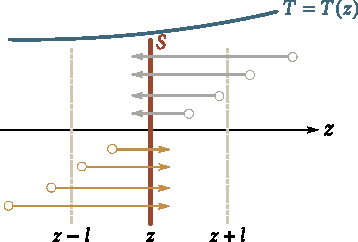
\includegraphics[scale=1]{figures/ch_16/fig_16_7.pdf}
		\caption[]{}
		\label{fig:16_7}
	\end{center}
\end{figure}

%On the basis of simplified notions, we shall consider that the number of mole-cules flying in one second through area $S$ in each direction (from left to right and from right to left) is
Để đơn giản hoá, ta coi như số phân tử xuyên qua diện tích $S$ theo một hướng trong một giây (từ trái sang phải và từ phải sang trái) là.
\begin{equation}\label{eq:16_20}
    N = \frac{1}{6} n \average{v} S.
\end{equation}

%At constant pressure, $n$ depends on the temperature ($p=nkT$), and $\average{v}$ also changes with the temperature. Accordingly, it would seem that to find the number of molecules flying through area $S$ from left to right we ought to use in \eqn{16_20} the values of $n$ and $\average{v}$ corresponding to one temperature, and to find the number of molecules flying from right to left, the values of $n$ and $\average{v}$ corresponding to another temperature. The numbers of molecules flying through area $S$ in opposite directions cannot differ, however. If they did, then apart from the heat flux through area $S$, we would also observe a flow of matter---the gas would be transported from one part of space to another. But we assumed that no processes occur in the gas except for the transport of heat. Therefore, we shall use \eqn{16_20} to calculate the number of molecules flying through $S$ in each direction, assuming for $n$ and $\average{v}$ their values in section $S$.
Với một áp suất không đổi, $n$ phụ thuộc vào nhiệt độ ($p=nkT$), và $\average{v}$ cũng thay đổi nếu thay đổi nhiệt độ. Vì vậy, ta coi như số phân tử xuyên qua diện tích $S$ từ trái sang phải được tính bằng cách thế các giá trị $n$ và $\average{v}$ tại một nhiệt độ xác định. Số phân tử xuyên qua diện tích $S$ theo chiều người lại thì cũng tương tự. Bởi vì nếu nó khác, thì ta không chỉ chứng kiến thông nhiệt lượng mà còn chứng kiến dòng vật chất---chất khí sẽ chuyển động từ nơi này sang nơi khác. Nhưng chúng ta giả thuyết rằng, không có quá trình nào khác ngoài sự vận chuyển nhiệt. Vì thế, chúng ta sẽ sử dụng \eqn{16_20} để tính số phân tử xuyên qua mặt $S$ với mỗi hướng, bằng cách tìm $n$ và $\average{v}$ các giá trị tại mặt $S$.

%It must be noted that since $n=p/kT$, \ie, $n$ is proportional to $p/T$, and $\average{v}$ is proportional to $\sqrt{T}$, the constancy of the product $n\average{v}$ signifies the constancy of the expression
Ta đã biết rằng $n=p/kT$, nên $n$ sẽ tỉ lệ thuận với $p/T$, và $\average{v}$ sẽ tỉ lệ thuận với $\sqrt{T}$, vì tích $n\average{v}$ không đổi nên biểu thức sau cũng không đổi
\begin{equation*}
    \frac{p}{T}\sqrt{T} = \frac{p}{\sqrt{T}}.
\end{equation*}

\noindent
%Hence, for no flow of molecules to be observed when a temperature gradient is present, it is essential that the pressure change along the $z$-axis in proportion to $\sqrt{T}$.
Vì vậy, để không có dòng dịch chuyển phân tử xảy ra cùng lúc có gradient nhiệt độ, thì điều quan trọng là áp suất thay đổi dọc theo trục $z$ tỉ lệ thuận với $\sqrt{T}$.
%In calculating the heat flux, we shall proceed from the assumption that every molecule carries with it the energy $\varepsilon=kT/2$ corresponding to the temperature at the spot where its last collision with another molecule occurred. On the average, this collision occurs at a distance from $S$ equal to the mean free path $l$ (see \fig{16_7}). Thus, the energy $\average{\varepsilon_1}$ corresponding to the temperature $T_1=T(z-l)$, \ie, to the temperature in the plane $(z-l)$, should be ascribed to the molecules flying in the direction of the $z$-axis, and the energy $\average{\varepsilon_2}$ corresponding to the temperature $T_2=T(z+l)$ should be ascribed to the molecules flying in the opposite direction (here $z$ is the coordinate of plane $S$).
Để tính toán thông lượng nhiệt, ta sẽ xuất phát từ giả thuyết rằng một phân tử mang một năng lượng $\varepsilon=kT/2$ tương ứng với nhiệt độ ở điểm mà tại đấy xảy ra va chạm với phân tử khác. Về trung bình, sự va chạm đó xảy ra cách đoạn $S$ bằng với quãng đường tự do trung bình $l$ (xem \fig{16_7}). Vì vậy, năng lượng $\average{\varepsilon_1}$ ứng với nhiệt độ $T_1=T(z-l)$, tức là nhiệt độ tại mặt phẳng $(z-l)$, sẽ được gán cho các phân tử bay cùng chiều trục $z$; năng lượng $\average{\varepsilon_2}$ ứng với nhiệt độ $T_2=T(z+l)$, sẽ được gán cho các phân tử bay ngược chiều trục $z$ (ở đây $z$ là toạ độ của mặt phẳng $S$).

%In accordance with the above, we get the following expression for the heat flux through area $S$ in the positive direction of the $z$-axis:
Theo những gì đã nói ở trên, chúng ta có được biểu thức thông lượng nhiệt qua mặt $S$ theo chiều dương của trục $z$:
\begin{equation*}
    q = N\parenthesis{\average{\varepsilon_1} - \average{\varepsilon_2}}
\end{equation*}

\noindent
%where $N$ is determined by \eqn{16_20}. Introduction of the values of $N$, $\average{\varepsilon_1}$, and $\average{\varepsilon_2}$ yields
Ở đây $N$ được xác định bởi \eqn{16_20}. Thế các giá trị $N$, $\average{\varepsilon_1}$, và $\average{\varepsilon_2}$ ta có
\begin{equation}\label{eq:16_21}
    q = \frac{1}{6} n\average{v} S \parenthesis{\frac{i}{2}kT_1 - \frac{i}{2}kT_2} = \frac{1}{6} n\average{v} S \frac{i}{2} k\parenthesis{T_1-T_2}.
\end{equation}

\noindent
%The difference $T_1-T_2$ equals
Hiệu $T_1-T_2$ bằng
\begin{equation}\label{eq:16_22}
    T (z-l) - T (z+l) = -\diff{T}{z} 2l
\end{equation}

\noindent
%(we have taken into account the smallness of $l$). Here $\diffin{T}{z}$ is the derivative of $T$ with respect to $z$ at the location of plane $S$.
(chúng ta đã lợi dụng việc $l$ rất nhỏ). Ở đây $\diffin{T}{z}$ là đạo hàm của $T$ theo $z$ tại điểm thuộc mặt $S$.

%With a view to \eqn{16_22}, we can write \eqn{16_21} as follows:
Để ý \eqn{16_22}, ta có thể viết \eqn{16_21} theo
\begin{equation}\label{eq:16_23}
    q = -\frac{1}{6} n\average{v} S \frac{i}{2}k\,\diff{T}{z} 2l = -\frac{1}{3} \average{v} l \parenthesis{\frac{i}{2}kn}\,\diff{T}{z} S.
\end{equation}

\noindent
%A comparison of this equation with \eqn{16_3} gives the following expression for the thermal conductivity coefficient:
Khi so sánh phương trình này với \eqn{16_3}, chúng ta rút ra được biểu thức cho hệ số dẫn nhiệt: 
\begin{equation}\label{eq:16_24}
    \varkappa = \frac{1}{3} \average{v} l \parenthesis{\frac{i}{2}kn}.
\end{equation}

%It should be remembered that the expression $iR/2=ik\ab{N}{A}/2$ determines the heat capacity at constant volume $C_V$ of one mole of a gas, \ie, the amount of a gas containing $\ab{N}{A}$ molecules. Similarly, the expression $ikn/2$ is the heat capacity of the amount of a gas containing $n$ molecules, \ie, the heat capacity of a unit volume of the gas. We can obtain this heat capacity by multiplying the specific heat capacity $c_V$ (the heat capacity of a unit mass) by the mass of a unit volume, \ie, by the density of the gas $\rho$. Thus,
Chúng nhớ lại rằng biểu thức $iR/2=ik\ab{N}{A}/2$ dùng để xác định hiện dung riêng đẳng tích $C_V$ của một mol khí, hay của một lượng khí chứa $\ab{N}{A}$ phân tử. Tương tự, biểu thức $ikn/2$ là nhiệt dung của lượng khí chứa $n$ phân tử, có thể hiểu là nhiệt dung riêng của một đơn vị thể tích. Chúng ta có thể thu được nhiệt dung này bằng cách nhân nhiệt dung riêng $c_V$ (nhiệt dung trên một đơn vị khối lượng) với khối lượng trên một đơn vị thể tích, hoặc có thể hiểu là mật độ khối lượng khí $\rho$. Như vậy
\begin{equation}\label{eq:16_25}
    \frac{i}{2}kn = \rho c_V.
\end{equation}

%Introducing \eqn{16_25} into~\eqref{eq:16_24}, we arrive at the final expression for the thermal conductivity coefficient of a gas:
Thế \eqn{16_25} vào \eqref{eq:16_24}, chúng ta đi đến biểu thức cuối cùng của hệ số dẫn nhiệt của chất khí: 
\begin{equation}\label{eq:16_26}
    \varkappa = \frac{1}{3} \average{v} l \rho c_V.
\end{equation}

\noindent
%As we have expected, the thermal conductivity coefficient was found to be proportional to $\average{v}, l$, and the heat capacity of a gas $\rho c_V$. More strict calculations lead to a similar expression for $\varkappa$, but with a somewhat different numerical factor.
Như chúng ta đã dự đoán, hệ số dân nhiệt tỉ lệ với $\average{v}, l$, và nhiệt dung của chất khí $\rho c_V$. Nếu tính toán chi tiết hơn chúng ta cũng sẽ có một biểu thức tương tự dành cho $\varkappa$, nhưng với một hệ số tỉ lệ chính xác hơn.

%Let us find how $\varkappa$ depends on the quantities characterizing molecules and on the parameters of state of a gas. Taking into account that $average{v}$ is proportional to $\sqrt{T/m}$, $l$ is proportional to $1/n\sigma$, and $\rho c_V$ is proportional to $in$ [see \eqn{16_25}], we get
Chúng ta giải thích sự phụ thuộc của $\varkappa$ vào các đại lượng đặc trưng cho phân tử và vào các tham số trạng thái của khí. Lưu ý rằng $\average{v}$ tỉ lệ với $\sqrt{T/m}$, $l$ tỉ lệ với $1/n\sigma$, và $\rho c_V$ tỉ lệ với $in$ [xem \eqn{16_25}], chúng ta có
\begin{equation}\label{eq:16_27}
    \varkappa \propto \parenthesis{\frac{T}{m}}^{1/2} \frac{1}{n\sigma} i n = \frac{i}{\sigma} \parenthesis{\frac{T}{m}}^{1/2}.
\end{equation}

%Inspection of expression~\eqref{eq:16_27} shows that unlike the diffusion coefficient, the thermal conductivity coefficient of a gas does not depend on the number of molecules in a unit volume, and, therefore, on the pressure ($p=nkT$). This is due to the following reasons. Reduction of the pressure is attended by diminishing of $n$, \ie, of the number of molecules participating in the transfer of energy. Simultaneously, $l$ grows and, consequently, also the difference between the energies transported by every molecule in opposite directions. As a result, we see that the amount of energy transferred by the molecules at the given temperature gradient does not depend on the pressure. This holds only as long as $l$ remains small in comparison with the distance between the surfaces exchanging heat at the expense of the thermal conductivity of the gas contained between them (for example, in comparison with the size of the gap between the internal and external walls of a glass vacuum bottle). As this condition stops being observed, the thermal conductivity begins to depend to a greater and greater extent on the pressure, diminishing when the latter lowers. When $l$ exceeds the distance between the surfaces, the path of the molecules is determined by the magnitude of this distance and stops depending on the pressure. The number of molecules per unit volume continues to fall off with decreasing pressure, the result being a reduction in $\varkappa$.
Từ biểu thức \eqref{eq:16_27} ta thấy rằng, khác với hệ số khuếch tán, hệ số dẫn nhiệt của chất khí không phụ thuộc vào số phân tử trong một đơn vị thể tích, và do đó không phụ thuộc vào áp suất (vì $p=nkT$). Điều trên có nguyên nhân sau đây. Khi giảm áp suất thì $n$ giảm, hay có thể hiểu là số phân tử tham gia vào việc vận chuyển năng lượng giảm. Cùng lúc đó, $l$ tăng và do đó sự chênh lệch năng lượng giữa hai dòng hạt ngược chiều nhau (xem \eqref{eq:16_22}). Kết quả là chúng ta thấy rằng năng lượng được truyền đi bởi các phân tử tại một gradient nhiệt độ xác định không phụ thuộc vào áp suất. Điều này chỉ đúng khi mà $l$ nhỏ so với khoảng cách giữa các mặt trao đổi nhiệt nhờ sự dẫn nhiệt của chất khí nằm giữa chúng (ví dụ, khi so sánh khoảng cách giữa vách trong và vách ngoài của một bình phích thuỷ tỉnh). Chừng nào mà điều kiện trên không còn được thoả mãn, thì hệ số dẫn nhiệt sẽ phụ thuộc mạnh vào áp suất, khi áp suất giảm thì hệ số cũng giảm. Khi mà $l$ lớn hơn khoảng cách giữa các mặt, thì quãng đường đi được của phân tử chính bằng độ lớn của khoảng cách giữa các mặt và không còn phụ thuộc vào áp suất. Số phân tử trong một đơn vị thể tích giảm khi giảm ấp suất, kết quả là $\varkappa$ cũng giảm. 

%When the temperature is raised, the thermal conductivity coefficient grows somewhat more rapidly than $\sqrt{T}$. The cause is that the effective section a depends slightly on $T$ (see \sect{16_2}).
Khi nhiệt độ được tăng lên, hệ số dẫn nhiệt sẽ tăng nhanh hơn một chút so với $\sqrt{T}$. Nguyên nhân là do tiết diện hiệu dụng $\sigma$ phụ thuộc ít vào $T$ (xem \sect{16_2}).

\section{Độ Nhớt của Chất Khí}\label{sec:16_5}

%To understand the origin of forces of internal friction, let us consider two contacting layers of a gas having a thickness of $\Delta z$. We shall assume that the layers move with different velocities $u_1$ and $u_2$ (\fig{16_8}). Every molecule of the gas participates in two motions: chaotic thermal motion whose mean velocity is $\average{v}$, and ordered motion with the velocity $u$ that is much smaller than $\average{v}$.
Để hiểu được sự xuất hiện về nội lực ma sát, ta xét hai lớp khí có độ dày $\Delta z$ tiếp xúc với nhau. Chúng ta giả thiết rằng các lớp khí di chuyển với tốc độ khác nhau $u_1$ và $u_2$ (\fig{16_8}). Mỗi phân tử khí tham gia vàoo hai chuyển động: chuyển động nhiệt hỗn loạn với vận tốc trung bình là $\average{v}$, và chuyển động có hướng với vận tốc $u$ rất nhỏ so với $\average{v}$.

\begin{figure}[!htb]
	\begin{center}
		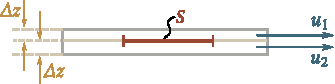
\includegraphics[scale=1]{figures/ch_16/fig_16_8.pdf}
		\caption[]{}
		\label{fig:16_8}
	\end{center}
\end{figure}

%Suppose that at a certain moment the layers have the momenta $K_1$ and $K_2$. These momenta cannot remain unchanged because owing to thermal motion the continuous transition of molecules from one layer to another occurs. According to our simplified notions, the number of molecules passing through area $S$ from one layer to another a second is determined by the expression
Giả sử rằng tại một thời điểm bất kì các lớp khí có động lượng $K_1$ và $K_2$. Các động lượng này không thể nào bảo toàn bởi vì chuyển động nhiệt nên liên tục có sự trao đổi phân tử từ lớp khí này sang lớp khí khác. Theo những khái niệm đã được đơn giản hoá, số phân tử đi qua diện tích $S$ từ lớp này sang lớp khác được xác định bởi biểu thức
\begin{equation}\label{eq:16_28}
    N = \frac{1}{6} n \average{v} S
\end{equation}

\noindent
%(the insignificant effect of ordered motion on the magnitude of the velocity of the molecules may be disregarded). Upon getting into another layer, a molecule collides with the molecules of that layer. As a result, it either gives up its surplus momentum to other molecules (if it arrived from a layer moving with a greater velocity), or increases its momentum at the expense of the other molecules (if it arrived from a layer moving with a smaller velocity). As a result, the momentum of the faster layer diminishes, and of the slower one grows. The layers thus behave as if a retarding force is applied to the first layer (whose velocity is greater), and an accelerating force equal in magnitude is applied to the second layer (whose velocity is lower).
(có thể bỏ qua ảnh hưởng của chuyển động lớp khí lên độ lớn vận tốc các phân tử khí)
Khi rơi vào lớp khí khác, một phân tử sẽ va chạm với một phân tử khác trong lớp khí đó. Vì thế, hoặc nó có thể trao động lượng dự trữ cho các phân tử khác (nếu nó đến từ lớp khí có vận tốc lớn hơn) hoặc có thể tăng động lượng của nó lên nhờ các phân tử khác (nếu nó đến từ lớp khí có vận tốc nhỏ hơn). Kết quả là, động lượng của lớp khí di chuyển nhanh hơn giảm đi, còn của lớp khí còn lại thì tăng lên. Đối với lại lớp khí có vận tốc lớn hơn, thì lực tác dụng lên nó là lực cản; với lớp khí có vận tốc nhỏ hơn, thì lực tác dụng lên nó là lực tăng tốc chuyển động.

%The momentum transferred through area $S$ on the interface between the layers depicted in \fig{16_8} in unit time from the first layer to the second one is
Động lượng được truyền từ lớp thứ nhất sang lớp thứ hai, xét trong một đơn vị thời gian, và qua diện tích $S$ tại mặt phân cách giữa hai lớp khí được thể hiện ở \fig{16_8}
\begin{equation*}
    K = N \parenthesis{mu_1 - mu_2}
\end{equation*}

\noindent
%($m$ is the mass of a molecule). Introduction of \eqn{16_28} for $N$ 
(với $m$ là khối lượng của phân tử). Thế giá trị của $N$ từ \eqn{16_28}
yields
\begin{equation}\label{eq:16_29}
    K = \frac{1}{6} n \average{v} S m \parenthesis{mu_1 - mu_2}.
\end{equation}

%In a real gas flow, the velocity when crossing the interface between two layers changes not in a jump, but continuously according to the law $u=u(z)$ (\fig{16_9}). We shall consider that every molecule flying through surface $S$ carries along with it the momentum $mu$ determined by the value of the velocity $u$ at the spot where the last collision of the molecule occurred. Different molecules experience their last collision at the most diverse distances from $S$. On the average, this collision occurs at a distance equal to the free path $l$. We shall therefore ascribe the velocity $u_1=u(z-l)$ to the molecules flying in the direction of the $z$-axis, and the velocity $u_2=u(z+l)$ to the molecules flying in the opposite direction. Inserting these values in \eqn{16_29}, we get the following expression for the momentum flux in the direction of the $z$-axis:
Đối với khí thực, vận tốc của phân tử khi đi qua mặt phân cắt không phải không có bước nhảy, nhưng thay đổi liên tục theo quy luật $u=u(z)$ (\fig{16_9}). Chúng ta coi rằng mỗi phân tử đi qua mặt $S$ đều mang một động lượng $mu$ được xác định bằng giá trị vận tốc $u$, tại điểm đó phân tử va chạm với nhau lần cuối. Các phân tử riêng biệt có khoảng từ điểm va chạm lần cuối đến $S$ khác nhau. Nhưng về trung bình, điểm diễn ra va chạm lần cuối sẽ có khoảng cách so với $S$ bằng quãng đường tự do trung bình $l$. Vì vậy ta viết được giá trị vận tốc $u_1=u(z-l)$ cho những phân tử đi theo chiều trục $z$, và giá trị vận tốc $u_2=u(z+l)$ cho những hạt đi theo chiều ngược lại. Thay các giá trị này vào \eqn{16_29}, ta sẽ có biểu thức cho thông lượng động lượng theo chiều của trục $z$.
\begin{equation*}
    K = \frac{1}{6} n \average{v} S m \bracket{u(z-l)-u(z+l)} = \frac{1}{6} n \average{v} S m\,\diff{u}{z} 2l
\end{equation*}

\noindent
%[compare with \eqn{16_23}].
[so sánh với \eqn{16_23}]

\begin{figure}[!htb]
	\begin{center}
		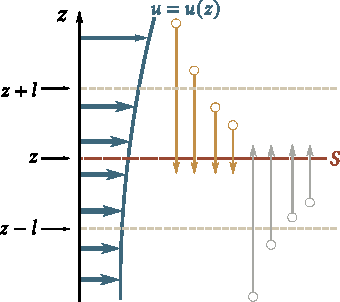
\includegraphics[scale=1]{figures/ch_16/fig_16_9.pdf}
		\caption[]{}
		\label{fig:16_9}
	\end{center}
\end{figure}

%Taking into account that the product nm equals the density of a gas $\rho$, we can write that
Nếu để ý, ta thấy rằng tích $n m$ bằng với khối lượng riêng của khí $\rho$, do đó ta có thể viết
\begin{equation*}
    K = -\parenthesis{\frac{1}{3} \average{v} l \rho}\,\diff{u}{z} S.
\end{equation*}

\noindent
%A comparison with \eqn{16_5} gives an expression for the viscosity:
Khi so sánh với \eqn{16_5} ta có thể rút ra được biểu thức cho hệ số nhớt
\begin{equation}\label{eq:16_30}
    \eta = \frac{1}{3} \average{v} l \rho.
\end{equation}

\noindent
%Stricter calculations lead to the same expression, but with a somewhat different numerical factor.
Tính toán chi tiết hơn sẽ dẫn đến cùng một biểu thức, nhưng với một hệ số chính xác hơn.

%It can he seen from \eqn{16_30} that like $D$ and $\varkappa$, the viscosity is proportional to $\average{v}$ and $l$. It is also proportional to the density of a gas $\rho$, \ie, to a quantity characterizing the ability of a gas to ``accumulate'' momentum---at a given velocity $u$ the momentum of a unit volume of a gas is the greater, the higher is the density $\rho$ (we remind our reader that the thermal conductivity is proportional to the heat capacity of a unit volume of a gas).
Có thể thấy từ \eqn{16_30} rằng $D$, $\varkappa$ và hệ số nhớt đều tỉ lệ thuận với $\average{v}$ và $l$. Ngoài ra, nó cũng tỉ lệ thuận với khối lượng riêng khí $\rho$, hay tức là với đại lượng đặc trưng cho khả năng ``tích luỹ'' động lượng --- tại một giá trị vận tốc nhất định, động lượng của một đơn vị thể tích càng lớn khi khối lượng riêng càng lớn ( ta hãy nhớ rằng hệ số dẫn nhiệt tỉ lệ thuận với nhiệt dung của một đơn vị thể tích khí).

%Taking into account the expressions for the quantities in \eqn{16_30}, we can write that
Để ý đến biểu thức của các đại lượng trong \eqn{16_30}, chúng ta có thể viết
\begin{equation*}
    \eta \propto \parenthesis{\frac{T}{m}}^{1/2} \frac{1}{n\sigma} n m = \frac{\sqrt{mT}}{\sigma}.
\end{equation*}

\noindent
%Hence, it follows that like $\varkappa$, the viscosity does not depend on the pressure. This holds only as long as $l$ remains small in comparison with the size of the gap through which the gas is flowing (for example, in comparison with the diameter of a pipe). As this condition stops being observed, the viscosity begins to depend more and more on the pressure, diminishing when the latter drops. The viscosity $\eta$ depends on the temperature in the same way as $D$ and $\varkappa$.
Từ đây suy ra rằng, cũng giống như $\varkappa$, hệ số nhớt không phụ thuộc vào áp suất. Nhưng điều này chỉ đúng khi mà $l$ là nhỏ khi so sánh với kích thước của hai vách bình mà khí đang chảy trong đó (chẳng hạn, so với đường kính của ống mà khí đang chảy). Nếu điều kiện này không còn được thoả mãn, thì hệ số nhớt bắt đầu phụ thuộc mạnh vào áp suất, lúc này hệ số nhớt giảm khi áp suất giảm. Hệ số nhớt $\eta$ phụ thuộc vào nhiệt độ giống như $D$ và $\varkappa$.

\section{Các Chất Khí Siêu Loãng}\label{sec:16_6}

%When the free path of molecules exceeds the linear dimensions of the vessel confining them, we say that a vacuum has been achieved in the vessel. The gas in this case is called \textbf{ultrararefied}. Although the word vacuum literally means ``emptiness'', an ultrararefied gas contains a great number of molecules in a unit volume. Thus, at a pressure of \SI{e-6}{\mmHg}, one cubic metre contains about \num{e16} molecules. Moreover, in very minute pores, the state defined as a vacuum can also be achieved at atmospheric pressure.
Khi quãng đường tự do của phân tử lớn hơn khoảng cách giữa hai vách bình chưa nó, ta có thể nói rằng trong bình đạt trạng thái chân không. Trong trường hợp này thì chất khí được gọi là \textbf{chất khí siêu loãng}. Mặc dù theo nghĩa đen thì chân không có nghĩa là ``rỗng không'', nhưng với chất khí siêu loãng vẫn còn chứa số lượng rất lớn các phân tử trong một đơn vị thể tích. Chẳng hạn, ở áp suất \SI{e-6}{\mmHg}, một mét khối chứa \num{e16} phân tử. Ngoài ra, khi xét các lỗ xốp rất nhỏ, trạng thái chân không cũng có thể đạt được, ngay cả khi dưới áp suất khí quyển.

%The behaviour of ultrararefied gases is distinguished by numerous features. For conditions of a vacuum, we cannot speak of the pressure of one part of a gas on another. In ordinary conditions, the molecules often collide with one another. Consequently, any surface with which we mentally divide a gas into two parts will experience an exchange of momenta between molecules. Thus, one part of the gas will act on the other with the pressure $p$ over the interface. In a vacuum, the molecules exchange momenta only with the wa1ls of the vessel, so that only the concept of the pressure of a gas on a wall has a meaning. Internal friction is also absent in the gas. But a body moving in an ultrararefied gas will experience the action of a friction force due to the fact that the molecules colliding with this body will change its momentum. Let us consider this in greater detail.
Biểu hiện của các chất khí siêu loãng nổi bật bởi một số tính chất. Trong điều kiện chân không, chúng ta không thể nói áp suất của phần khí này lên phần khí khác. Trong điều kiện thông thường, các phân tử thường va chạm với nhau. Kết quả là, với một mặt diện tích bất kì mà ta chọn, ở đấy có sự trao đổi động lượng hai bên chất khí. Do đó, một phần chất khí sẽ tác dụng một áp suất $p$ lên phần còn lại tại mặt phân cách. Trong chân không, những phân tử chỉ trao đổi động lượng với thành bình, thế nên chỉ có khái niệm áp suất của khí lên thành bình có ý nghĩa. Nội ma sát cũng không tồn tại trong chất khí. Nhưng nếu vật chuyển động chất khí siêu loãng sẽ bị chịu một lực cản do các phân tử khí va chạm với vật và làm thay đổi động lượng của vật. Chúng ta sẽ xem xét vấn đề này kĩ hơn.

%Assume that two plates are moving parallel to each other in an ultrararefied gas (\fig{16_10}). The velocities of the plates are  $u_1$ and $u_2$. The interaction between a molecule and a plate at the moment of a collision leads to the molecule, upon rebounding from the plate, having a velocity component equal in magnitude and direction to the velocity of the plate in addition to its thermal velocity.
Xét hai tấm di chuyển song song với nhau trong một chất khí siêu loãng (\fig{16_10}). Vận tốc của các tấm lần lượng là $u_1$ và $u_2$. Tương tác của một phân tử với một tấm trong lúc va chạm sẽ dẫn đến sự kiện phân tử bị bật ra khỏi tấm, điều này sẽ bổ sung thêm một thành phần vận tốc khác, bên cạnh vận tốc chuyển động nhiệt. Thành phần này có độ lớn và phương chiều của vận tốc tấm.

%A unit area of the upper plate will be struck in one second by $n\average{v}/6$ molecules having a velocity component $u_2$ acquired in the preceding collision with the lower plate. Each of these molecules carries a momentum component of $mu_2$. Upon rebounding from the upper plate, the molecules have a momentum component of $mu_1$.
Trong một giây sẽ có $n\average{v}/6$ phân tử đập vào một đơn vị diện tích; những phân tử sẽ mang vận tốc $u_2$ mà nó nhận được khi va chạm với tấm dưới. Mỗi một phân tử này mang một thành phần động lượng $mu_2$. Sau khi va chạm với tấm trên, phân tử sẽ có thành phần động lượng là $mu_1$.

%Consequently, a collision of every molecule with the upper plate results in its momentum diminishing by $m\parenthesis{u_1-u_2}$. The change in the momentum in unit time related to unit surface area of the plate is
Kết quả là mỗi va chạm của các phân tử với tấm trên sẽ dẫn đến sự giảm động lượng $m\parenthesis{u_1-u_2}$. Sự biến thiên động lượng trong một đơn vị thời gian đối với một đơn vị bề mặt là
\begin{equation*}
    \frac{1}{6} n \average{v} m \parenthesis{u_1-u_2}.
\end{equation*}

\noindent
%This change equals the force acting on a unit surface area of the plate:
Sự biến thiên này bằng với lực tác dụng lên một đơn vị diện tích của tấm:
\begin{equation}\label{eq:16_31}
    F = \frac{1}{6} \rho \average{v} \parenthesis{u_1-u_2}
\end{equation}

\noindent
%(we have substituted $p$ for $nm$). A force of the same magnitude, but opposite in direction, acts on a unit surface area of the lower plate.
(chúng ta đã thay $\rho$ bằng $nm$). Một lực với cùng độ lớn, nhưng ngược chiều tác dụng lên một đơn vị diện tích của tấm dưới là.

%It is natural to call the proportionality constant between the force of friction and the velocity difference of the plates the coefficient of friction. It can be seen from \eqn{16_31} that this coefficient equals $\rho\average{v}/6$, \ie, is proportional to the density of the gas and, consequently, to the pressure of the gas on a plate and the walls of the vessel (the expression $p=nkT$ remains in force for this pressure).
Hệ số tỉ lệ giữa lực ma sát và hiệu vận tốc hai tấm dĩ nhiên được gọi là hệ số ma sát. Có thể thấy từ \eqn{16_31} rằng hệ số này bằng với $\rho\average{v}/6$, tức là nó tỉ lệ mật độ khối lượng của khí, kết quả là, cũng tỉ lệ thuận với áp suất trên bản và trên thành bình (đối với áp suất này $p=nkT$ vẫn bảo toàn).

\begin{figure}[!htb]
	\begin{minipage}[t]{0.5\linewidth}
		\begin{center}
			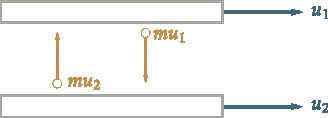
\includegraphics[scale=1]{figures/ch_16/fig_16_10.pdf}
			\caption[]{}
			\label{fig:16_10}
		\end{center}
	\end{minipage}
	\hspace{-0.05cm}
	\begin{minipage}[t]{0.5\linewidth}
		\begin{center}
			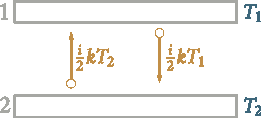
\includegraphics[scale=1]{figures/ch_16/fig_16_11.pdf}
			\caption[]{}
			\label{fig:16_11}
		\end{center}
	\end{minipage}
\end{figure}

%Let us now consider the transfer of heat by a gas in a vacuum. We shall consider two plates with temperatures $T_1$ and $T_2$ between which there is an ultrararefied gas (\fig{16_11}). If the impact of the molecules against the surface of the rigid body were of a perfectly elastic nature, the molecules would rebound from a plate with the same velocity in magnitude (and, consequently, with the same energy) as they had before the collision. As a result, the molecules would not be able to transfer energy from one plate to the other. Such a conclusion, however, contradicts experimental data. Hence, the interaction between a wall and a molecule striking it is not an elastic collision in nature. Indeed, it occurs as follows: upon striking a wall, a molecule adheres to it, as it were, for a brief time, after which it leaves the wall in an absolutely arbitrary direction with a velocity whose magnitude on the average corresponds to the temperature of the wall\footnote{We must note that this more precise definition of the nature of interaction of the molecules with a wall does not affect the results which we obtained in \sect{11_4} when calculating the pressure. If the temperature of the gas and the walls is the same, then the molecules will leave a wall with the same mean velocity with which they collided with it, so that the change in the momentum of the molecules as a result of a collision is the same on an average as in a perfectly elastic collision.}.
Chúng ta sẽ xét sự truyền nhiệt của chất khí trong điều kiện chân không. Chúng ta xét hai tấm với nhiệt độ lần lượt là $T_1$ và $T_2$, giữa chúng có một chất khí siêu loãng (\fig{16_11}). Nếu va chạm của phân tử với vật rắn là tuyệt đối đàn hồi, thì phân tử phải bật ra với cùng một tốc độ (và do đó, cùng năng lượng) so với trước khi phân tử va chạm. Và nếu như thế, phân tử sẽ không thể truyền năng lượng từ tấm này sang tấm khác. Tuy nhiên điều này rất mâu thuẫn với kết quả thực nghiệm. Vì vậy tương tác giữa thành bình và phân tử không phải là va chạm tuyệt đối đàn hồi. Trong thực tế, tương tác đó xảy ra như sau: sau khi va chạm với thành bình, hình như phân tử bị dính lại trên thành, trong một thời gian ngắn sau đó thì bị bật ra với một hướng bất kì, với tốc độ có giá trị trung bình tương ứng với nhiệt độ thành bình\footnote{Chú ý rằng, định nghĩa chính xác hơn của tương tác của phân tử và thành bình không ảnh hưởng đến kết quả áp suất mà chúng ta đã tính trong \sect{11_4}. Nếu nhiệt độ của khí và thành bình bằng nhau thì vận tốc phân tử rời khỏi thành bình sẽ bằng với vận tốc trước va chạm; vì thế nên sự biến thiên động lượng của phân tử, về trung bình, cũng giống trường hợp va chạm tuyệt đối đàn hồi.}

%Let us revert to \fig{16_11}. Each of the $n\average{v}S/6$ molecules striking the upper plate a second carries the energy $ikT_2/2$ along with it and carries away an energy of $ikT_1/2$. Hence, each impact of a molecule against a plate leads to the latter losing the energy $ik\parenthesis{T_1-T_2}/2$. The second plate receives the same energy upon each impact. Thus, the amount of energy transferred by the molecules in one second from plate to plate will be
Chúng ta hãy quay lại \fig{16_11}. Với $n\average{v}S/6$ phân tử đâm vào tấm trên trong một giây mang năng lượng $ikT_2/2$ và mang rời đi năng lượng là $ikT_1/2$. Do đó mỗi va chạm vào tấm sẽ dẫn đến sự mất mát năng lượng $ik\parenthesis{T_1-T_2}/2$. Tấm thứ hai sẽ nhận một năng lượng tương tự với mỗi sự va chạm. Vì thế, năng lượng được truyền đi bởi các phân tử trong một giây từ tấm này đến tấm khác là
\begin{equation*}
    q = \frac{1}{6} n \average{v} \frac{i}{2} k \parenthesis{T_1-T_2} S.
\end{equation*}

\noindent
%Multiplying and dividing this expression by $m\ab{N}{A}$, we get
Nhân và chia biểu thức với $m\ab{N}{A}$, ta có
\begin{equation}\label{eq:16_32}
    q = \frac{1}{6} \rho \average{v} c_V \parenthesis{T_1-T_2} S.
\end{equation}

%The thermal conductivity coefficient equal to $\rho\average{v}c_V/6$ is found to be proportional to the density of a gas when the latter is ultrararefied. Hence, heat transfer from one wall to another will fall off with decreasing pressure, whereas the thermal conductivity of a gas in ordinary conditions does not depend, as we have seen, on the pressure.
Hệ số truyền nhiệt bằng với $\rho\average{v}c_V/6$ sẽ tỉ lệ với mật độ khối lượng của khí nếu chất khí đó là siêu loãng. Do đó, khi giảm áp suất thì sự truyền nhiệt từ thành này sang thành kia cũng giảm. Trong khi đó, ta thấy rằng hệ số dẫn nhiệt của khí tại điều kiện thường thì không phụ thuộc vào áp suất.
